\chapter{Installation/Benutzung}
\label{cha:Installation/Benutzung}

\section{Deployment Diagramm}

\begin{figure}[hbt]
	\centering
	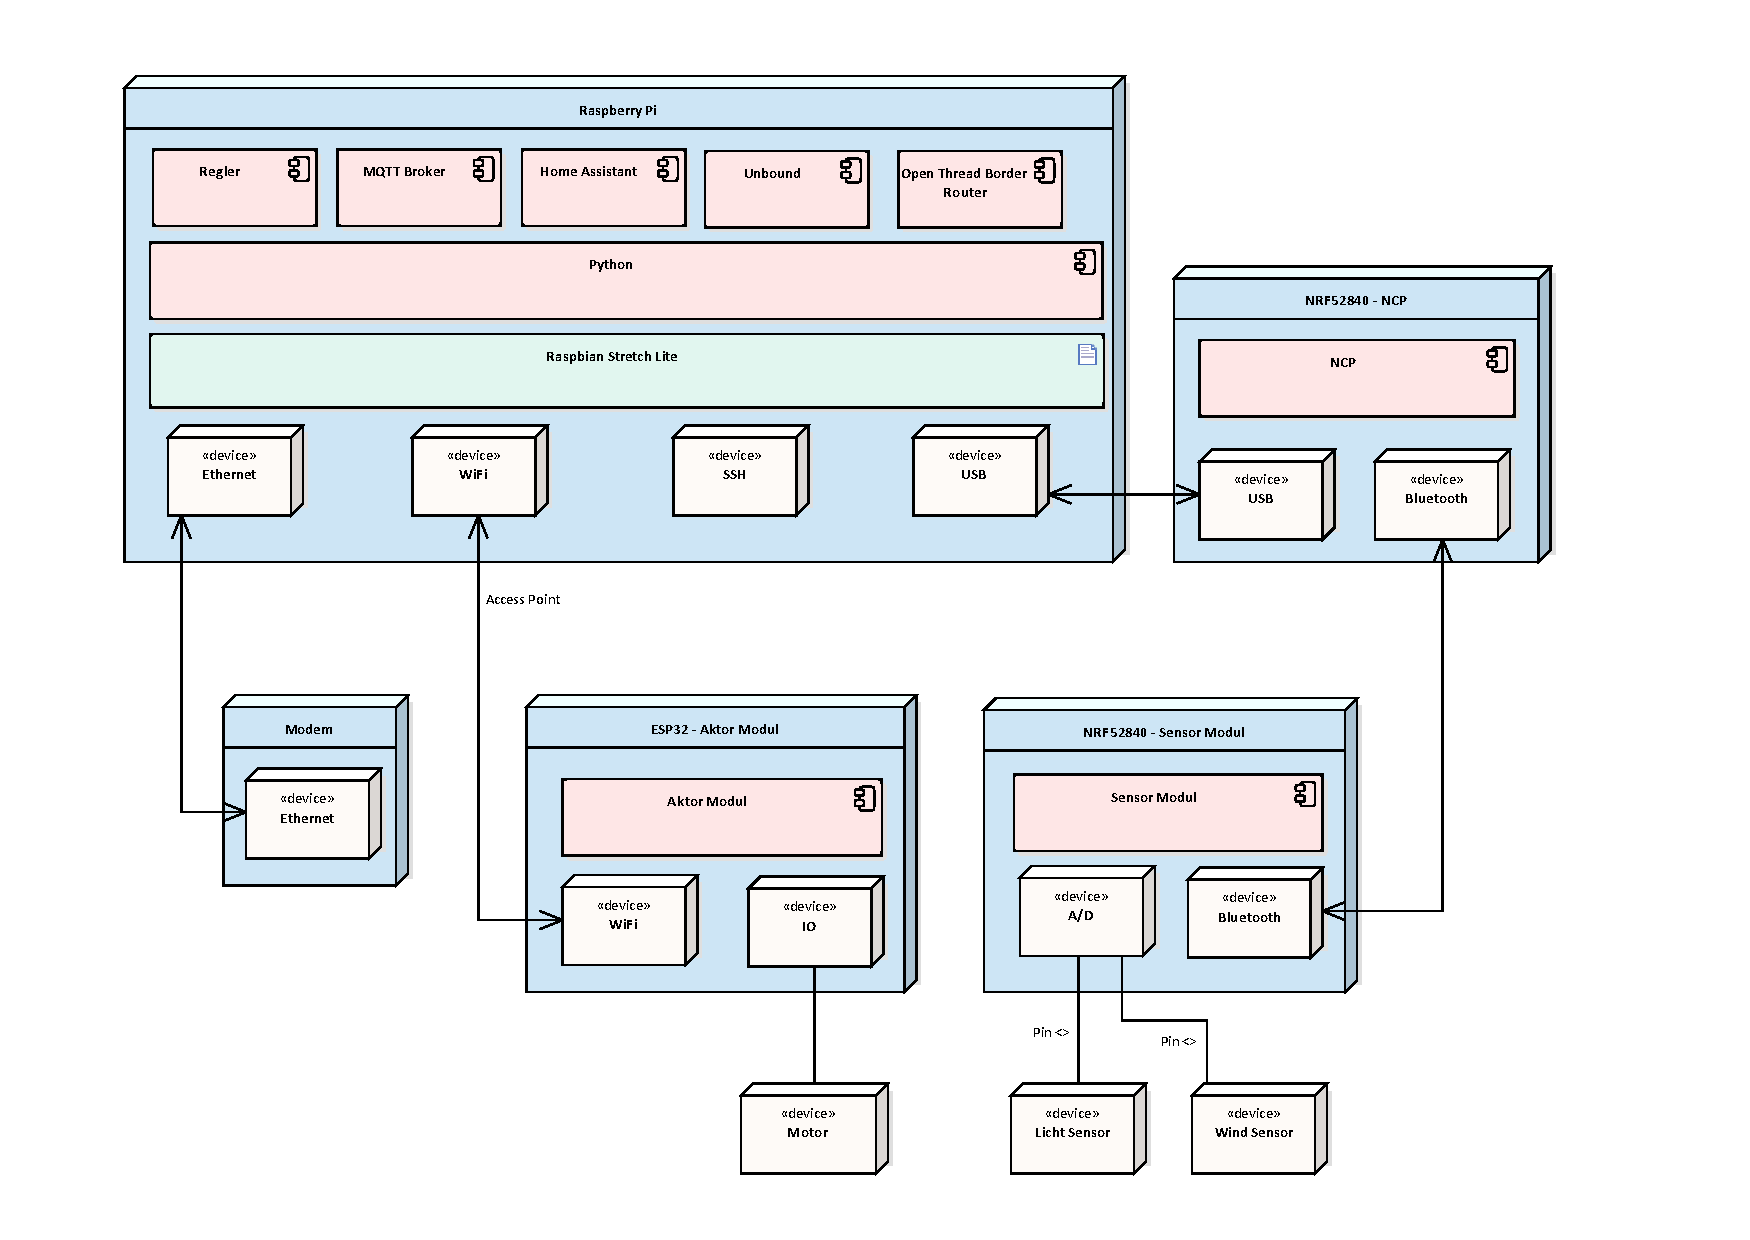
\includegraphics[width=1\linewidth]{images/Deployment}
	\caption[Deployment Diagramm]{Deployment Diagramm.}
	\label{fig:deployment_diagramm}
\end{figure}

Abbildung~\ref{fig:deployment_diagramm} zeigt das Deployment Diagramm des Systems. Im Folgenden wird einzeln auf die Installation der Module eingegangen.

\section{Sensor und Aktor Modul (ESP32)}
\label{cha:Installation_IDF}
\subsection{Schritt 1: Installation der ESP IDF}
Um die ESP32 Mikrocontroller flashen zu können, muss zunächst die Espressif IoT Development Framework (ESP IDF)\nomenclature{ESP IDF}{Espressif IoT Development Framework} installiert und eingerichtet werden. An dieser Stelle sei auf die \href{https://docs.espressif.com/projects/esp-idf/en/latest/index.html}{Dokumentation von Espressif} hingewiesen, um die Programmierumgebung abhängig vom Betriebssystem richtig einzurichten.

\subsection{Schritt 2: Anpassung der Konfiguration}
Der Quellcode für beide Module kann auf Github heruntergeladen werden: \href{https://github.com/maxbachmann-university/esp32-sensor-modul}{Sensor Modul}, \href{https://github.com/maxbachmann-university/esp32-actuator-module}{Aktor Modul}.
Anschließend wechselt man mit der Konsole in das jeweilige Verzeichnis. Mit dem Befehl \textbf{''make menuconfig''} wird die Konfiguration vorgenommen. Es öffnet sich ein Dialog, wie in Abbildung~\ref{fig:config_start} dargestellt. Unter dem ersten Menüpunkt kann der Port festgelegt werden, an welchen der ESP32 am Computer angeschlossen wurde. Unter ''Example Configuration'' können wie in Abbildung~\ref{fig:config_default} gezeigt die Verbindungsdaten des WLAN, des MQTT Brokers und des OTA Servers angepasst werden. Diese Konfiguration wird anschließend gespeichert.

\begin{figure}[hbt]
	\centering
	\includegraphics[width=0.8\linewidth]{images/make_menuconfig_start}
	\caption[Konfiguration Startseite]{Startseite der Konfiguration.}
	\label{fig:config_start}
\end{figure}

\begin{figure}[hbt]
	\centering
	\includegraphics[width=0.8\linewidth]{images/make_menuconfig_default}
	\caption[Konfiguration Standard]{Default Werte der Konfiguration.}
	\label{fig:config_default}
\end{figure}

\subsection{Schritt 3: Flashen}
Im letzten Schritt wird mit dem Befehl \textbf{''make flash''} der Mikrocontroller geflashed.

\section{Regler Modul (Raspberry PI)}

\subsection{Schritt 1: Installation von Raspbian}
Zunächst muss das image der aktuellsten Version von \href{https://www.raspberrypi.org/downloads/raspbian/}{Raspbian} auf die SD-Karte des Raspberry PI geladen werden.

\subsection{Schritt 2: MQTT Broker}
Für den MQTT Broker kann im Grunde jeder Beliebiger verwendet werden. Wir haben hierfür \href{http://mosquitto.org/}{Mosquitto} benutzt. Dieser Broker kann mit dem Befehl in Listing~\ref{lst:installmosquitto} installiert werden und läuft sofort.

\lstset{caption={Installation von Mosquitto.}}
\lstset{label={lst:installmosquitto}}
\begin{lstlisting}
sudo apt-get install -y mosquitto mosquitto-clients
\end{lstlisting}

\subsection{Schritt 3: Hinzufügen des Python Skripts}
Für die Regelung wird ein \href{https://github.com/maxbachmann-university/blind-controller}{Python Skript} verwendet, welches auch auf Github zu finden ist. Dieses kann in einem beliebigen Ort auf dem Raspberry Pi gespeichert werden, inklusive der ''config.yml'' Datei. In dieser können die Zugangsdaten zu dem MQTT Broker angepasst werden. Für den Autostart des Skripts beim Neustart, muss mit Hilfe des Befehls wie in Listing~\ref{lst:rc.local} im Terminal der Texteditor der Datei ''rc.local'' aufgerufen werden. Anschließend wird die Datei vor der Zeile ''exit 0'' um eine weitere Zeile ergänzt, in die nach einem ''python'' der Pfad zu dem Python Skript angegeben wird, gefolgt von einem ''\&''. Das ganze sieht dann zum Beispiel so aus, wie in Listing~\ref{lst:autostart}.

\lstset{caption={Öffnen der Autostart Datei im Editor Nano.}}
\lstset{label={lst:rc.local}}
\begin{lstlisting}
sudo nano /etc/rc.local
\end{lstlisting}

\lstset{caption={Anpassung der Autostart Datei.}}
\lstset{label={lst:autostart}}
\lstset{language=Python}
\begin{lstlisting}
python3 /home/pi/controller.py &
exit 0
\end{lstlisting}